\section{System Tuning and Experimental Results}

\begin{frame}{Tuning Kalman Filter Gains}

Tuning the Kalman Filter gains remains time consuming
\begin{enumerate}
	\item Tune \textbf{mobile phone} IMU and GPS noise variances by running and walking along known trajectories
	\item Tune gains related to \textbf{MAV INS} through experiments landing on static target, following phone, etc
	\item AprilTag detection and estimation by \textbf{gimbaled and fixed cameras}: 
	compare output to baseline provided by MoCap
	\item Filter tuning as a whole through full landing experiments
\end{enumerate}

\end{frame}

%\subsection{Tuning System Gains}
%\begin{frame}{\thesection. \insertsection \ - \insertsubsection}
%\begin{frame}{Tuning System Gains}
%	Tuning the Kalman Filter gains remains time consuming %difficult and
%	\begin{enumerate}
%		\item Gather baseline data for the \textbf{mobile phone}. Run and walk in a straight line,
%		circle, square, etc.
%		\item Tune corresponding noise parameters for IMU and GPS position, speed and velocity data
%		until the estimated trajectory is accurate.
%	\end{enumerate}
%\end{frame}

% ----------------------------------------------------------------------

%\begin{frame}{\thesection. \insertsection \ - \insertsubsection}
%\begin{frame}{Tuning System Gains II}
%	\begin{enumerate}
%		\setcounter{enumi}{2}
%		\item Gather baseline flight data: Land on a static mobile phone, follow
%		phone and land on a moving phone.
%		\item Tune gains relating to the MAV INS and review mobile phone tuning until
%		the data reflects the flight test.
%	\end{enumerate}
%	No vision sensors yet!
%\end{frame}

% ----------------------------------------------------------------------

%\begin{frame}{\thesection. \insertsection \ - \insertsubsection}
%\begin{frame}{Tuning System Gains III}
%	\begin{enumerate}
%		\setcounter{enumi}{4}
%		\item Tune the gains for the vision sensors i.e. AprilTag detection by the gimbaled and fixed cameras.\\
%		We used a motion capture system to compare ground truth data and the filter's output.
%		\item \textbf{Final step} : Tune the filter as a whole on full landing tests and make sure 
%		there are no regressions on the baseline data. The goal is to tune the relative weights of all
%		sensors w.r.t each other.
%		
%	\end{enumerate}
%\end{frame}

% ----------------------------------------------------------------------

%\begin{frame}{\thesection. \insertsection \ - \insertsubsection}
\begin{frame}{Tuning Controller Gains}
	Tuning the controller gains is easier than the estimator gains
	\begin{itemize}
		\item We use DJI's proprietary simulator to simulate the approach and landing phases in order to tune
		the PN controller, the switching distance and the PD controller
		\vspace{0.5cm}
		\item Flight tests for validation and testing under windy conditions
	\end{itemize}
\end{frame}

% ----------------------------------------------------------------------


%\begin{frame}{\thesection. \insertsection}
\begin{frame}{Experimental Results}
	\begin{figure}
		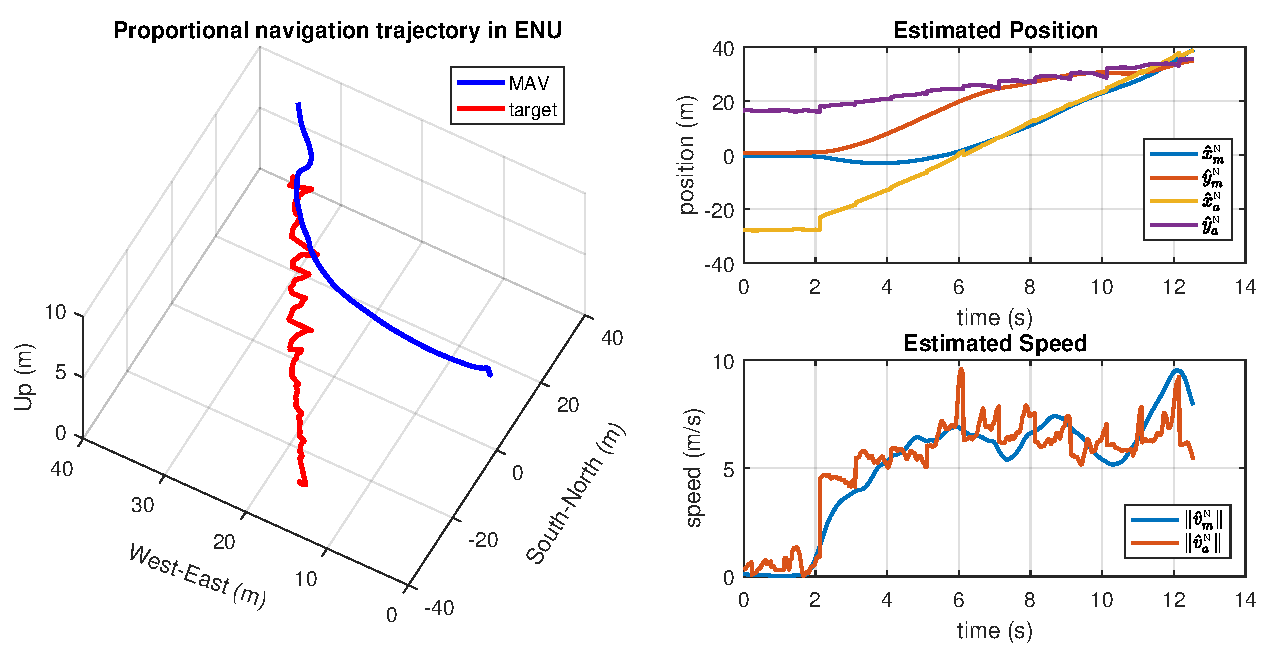
\includegraphics[width=0.8\paperwidth]{figures/pn.pdf} \\
		%\caption{
		Straight line trajectory test of the PN controller%}
	\end{figure}
\end{frame}

% ----------------------------------------------------------------------

%\begin{frame}{\thesection. \insertsection}
\begin{frame}{Experimental Results II}
	\begin{figure}
		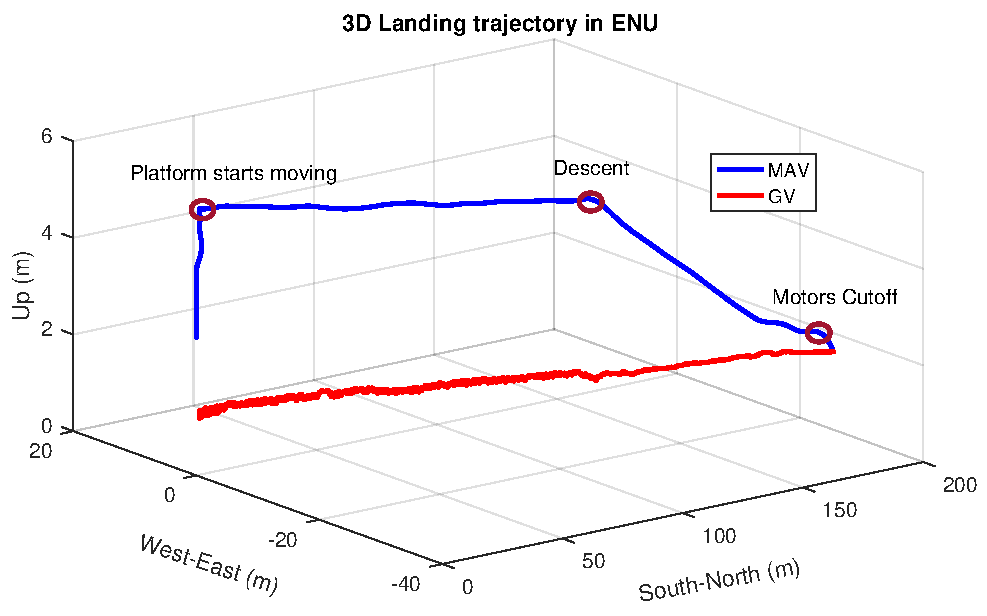
\includegraphics[width=0.8\paperwidth]{figures/landing.pdf} \\
		%\caption{
		%Side view of the 
		MAV landing on a moving car at 50 km/h with only the close range controller%}
	\end{figure}
\end{frame}

% ----------------------------------------------------------------------

%\begin{frame}{\thesection. \insertsection \ - \insertsubsection}
\begin{frame}{Experimental Results III}
	\begin{figure}
		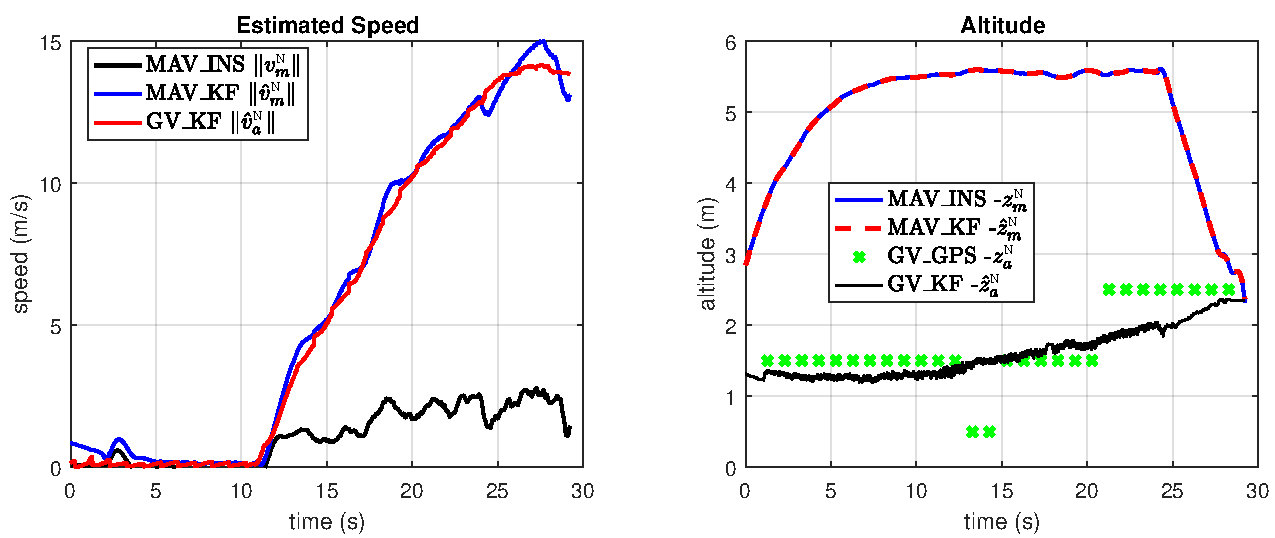
\includegraphics[width=0.8\paperwidth]{figures/landing_motion.pdf} \\
		%\caption{
		%Kalman filter outputs during flight. 
		%Notice the 
		INS' velocity output is invalid when the MAV is on top of the landing platform%.}
	\end{figure}
\end{frame}

% ----------------------------------------------------------------------

%\begin{frame}{\thesection. \insertsection}
\begin{frame}{Landing Examples}
	
	\begin{center}
	\includemedia[
			%width=0.4\linewidth,
	  		%totalheight=0.225\linewidth,
	  		%activate=pageopen,
			%final,
			playbutton=plain, %none,
	  		passcontext,  %show VPlayer's right-click menu
	  		addresource=figures/approachPhase.mp4,
	  		flashvars={
	    		%important: same path as in `addresource'
	    		source=figures/approachPhase.mp4
			}
	]{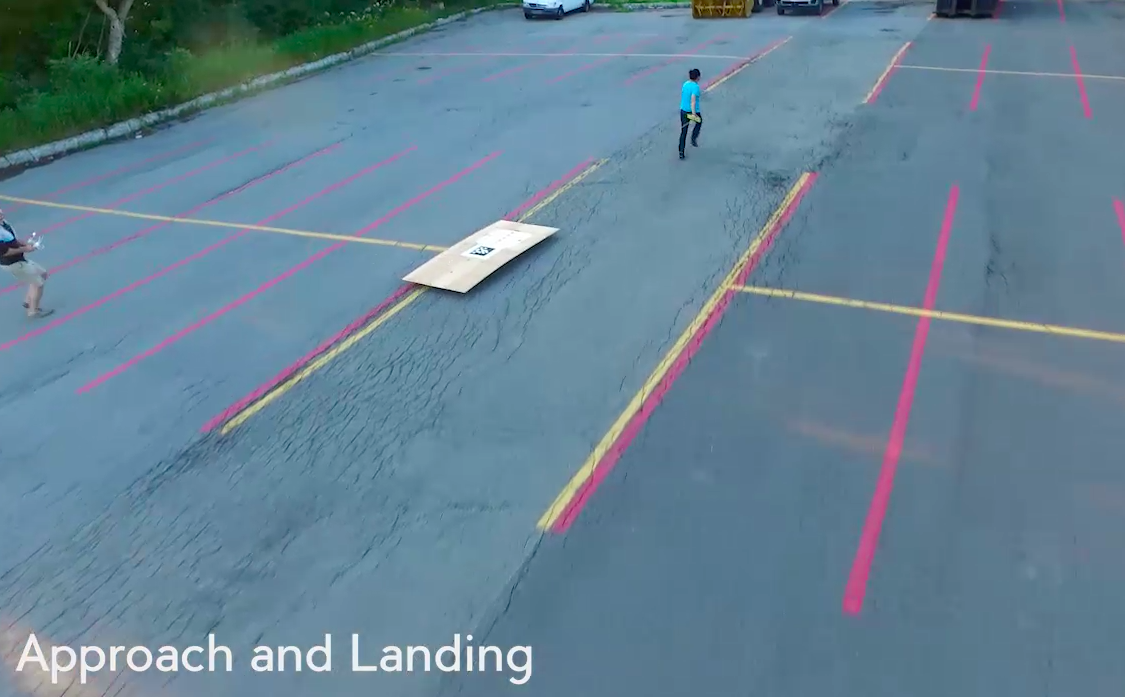
\includegraphics[width=0.8\paperwidth]{figures/landingPoster.png}}{VPlayer.swf}
	\end{center}
	
\end{frame}

% ----------------------------------------------------------------------

%\begin{frame}{\thesection. \insertsection}	
%	Why did it slip at $50$ km/h ?
%	\begin{enumerate}
%		\item Close to top speed of the MAV 
%		\item We introduced a small delay before motor cutoff to allow the MAV to straighten out.
%		\item At these speeds, airflow around the car becomes significant.
%	\end{enumerate}
%	The last two points combined give the MAV just enough lift to slide backwards.
%\end{frame}